\documentclass[10pt,a4paper]{article}

%double si on veut une version prof et une version élève. simple si on veut une seule version.
\newcommand{\buildmode}{double}

\InputIfFileExists{version.tex}{}{}
% Version (définie par le script)
\providecommand{\version}{eleve}

\usepackage{feuilleexo}

%%%à modifier à chaque fois

\renewcommand{\niveau}{1G}
\renewcommand{\chapitre}{Fonctions, généralités}
\renewcommand{\numchap}{0} 
\renewcommand{\theme}{Fonctions}

\begin{document}





%\legendeicones

\vspace{-0.3cm}

\begin{prerequis}
\begin{itemize}
    \item Connaître le vocabulaire d'une fonction : image, antécédent, sens de variation, extremum.
    \item Lire et compléter un tableau de valeurs, placer des points dans un repère.
    \item  Résoudre une équation du premier degré,  une inéquation du premier degré, une équation produit nul.
    \item Développer et factoriser une expression algébrique (double distributivité, identités remarquables).
    
    
\end{itemize}
\end{prerequis}

\begin{multicols}{2}

\section{Représentation graphique}

\begin{exo}[Rappels][]
On considère une fonction \(f\) dont la représentation graphique est donnée ci-dessous.

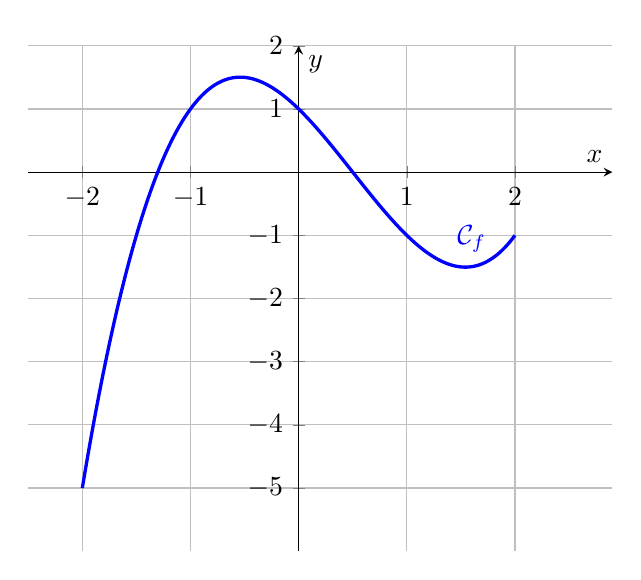
\begin{tikzpicture}
\begin{axis}[
    axis lines=middle,
    xmin=-2.5, xmax=2.9,
    ymin=-6, ymax=2,
    domain=-2:2,
    samples=300,
    grid=major,
    xtick={-2,-1,0,1,2,3},
    ytick={-5,-4,-3,-2,-1,0,1,2,3,4},
    xlabel={\(x\)},
    ylabel={\(y\)},
    width=9cm,
    height=8cm
]

\addplot[
    blue,
    very thick
] {2/3*(x-2)*(x+1.5)*(x-1)-1}
node[pos=0.92, above right] {\(\mathcal{C}_f\)};

\end{axis}
\end{tikzpicture}

\begin{enumerate}[leftmargin=*]
    \item Quel est l'ensemble de définition de \(f\) ?
    \item Donner les images de \(-2\), \(0\) et \(1\) par \(f\).
    \item Donner les éventuels antécédents de -1 et de 1.
    \item Résoudre \(f(x)=0\).
    \item Établir le tableau de signes de \(f\) sur son ensemble de définition.
    \item Résoudre \(f(x) \geq 0\).
    \item Dresser le tableau de variations de \(f\) sur son ensemble de définition.
    \item Le point de coordonnées \((-2;-5)\) appartient-il à \(\mathcal{C}_f\) ?
\end{enumerate}
\end{exo}


\begin{exo}[][appro]
    
On donne le tableau de signe suivant :

\begin{center}
\begin{tikzpicture}
\tkzTabInit[lgt=1.1,espcl=1.3]{\(x\) /1, \(f(x)\) /1}{\(-4\),\(-2\),\(1\),\(3\),\(5\)}
\tkzTabLine{,+,0,-,0,+,0,-,}
\end{tikzpicture}
\end{center}

Tracer une fonction admettant ce tableau de signes.
\end{exo}

\begin{exo}[][appro]
On donne le tableau de variations suivant :

\begin{center}
\begin{tikzpicture}
\tkzTabInit[lgt=1.1,espcl=1.3]{\(x\) /1, \(f\) /2}{\(-4\),\(0\),\(4\),\(5\)}
\tkzTabVar{+/\(4\),-/\(-2\),+/\(6\),-/\(-2\)}
\end{tikzpicture}
\end{center}

Tracer une fonction admettant ce tableau de variations.
\end{exo}

\begin{exo}[][avance]
    Est-il possible de tracer une fonction ayant pour tableaux de signe et de variations les deux tableaux ci-dessus ? Justifier.
\end{exo}

\prof{
    Contradiction non évidente pour des élèves en début de première. Plusieurs méthodes possibles :
   
   \smallskip

    - Remarquer que la valeur en 4 est négative dans le premier tableau et positive dans le 2e.

    \smallskip
    
    - Approche intuitive du TVI.
}

\begin{exo}[][appro]
    Tracer la courbe représentative \(\mathcal{C}_g\) de la fonction affine \(g\) telle que \begin{itemize}
        \item L'image de -1 est 4 ;
        \item Le point de coordonnées (1, 0) appartient à \(\mathcal{C}_g\)
    \end{itemize}
\end{exo}


    \section{Fonctions affines}

\begin{exo}[Rappels][]
On considère la fonction affine \(f\) définie sur \(\left[-4;9\right]\) par \(f(x)=2x+1\).

\begin{enumerate}[leftmargin=*]
    \item Quel est le sens de variation de \(f\).
    \item Déterminer le (ou les) antécédent(s) de \(0\).
    \item Tracer l'allure de la représentation graphique de \(f\).
    
    \smallskip

    \textit{i.e : faire apparaître graphiquement le signe du coefficient directeur et de l'ordonnée à l'origine.}
    \item Dresser le tableau de signe de \(f\).
    
    \smallskip
    
    \textit{Remarque : cela revient à résoudre l'inéquation \(f(x)\geq 0\).}
\end{enumerate}
\end{exo}
\prof{\begin{itemize}
    \item Laisser le choix de la méthode pour la question 4. 
    \item Pendant la phase de correction, détailler très clairement les deux méthodes. C'est un exemple du cours. Ils doivent savoir utiliser les deux pour les exercices suivants.
    \item Faire remarquer que dresser un tableau de signe revient à résoudre une inéquation. Expliciter que l'on peut y arriver par plusieurs méthodes (par le calcul, ou par le calcul et en utilisant un argument géométrique).
    \item Pour les variables didactiques : On commence qu'avec des nombres positifs. $f(x) = 2x+1$ donne $x=-\frac{1}{2}$. Cela permet de revoir la valeur décimale de $\frac{1}{2}$.
\end{itemize}
}

\begin{exo}[][]

    Les fonctions affines suivantes sont toutes définies sur \(\mathbb{R}\). Pour chacune d'entre elles, établir son tableau de signes par les deux méthodes vues dans l'exercice précédent.

    \begin{tasks}(2)
        \task \(f(x)= 4x-3\)
        \task \(g(x)= -5x+1\)
        \task \(h(x)= x+4\)
        \task \(i(x)= -x-2\)
    \end{tasks}
    
\end{exo}

\prof{
 \begin{itemize}
    \item Solutions des équations permettent de revoir les valeurs des fractions de références.
    \item Demander explicitement à ce qu'ils tracent approximativement la courbe représentative.
    \item Détailler \(\frac{3}{4}=3\times\frac{1}{4}=3\times 0.25=0.75\)
\end{itemize}
}

\begin{exo}[][appro]
    Soit \(m\) et \(p\) deux nombres réels strictement positifs. On considère la fonction affine \(f\) définie sur \(\mathbb{R}\) par \(f(x)=mx+p\).

    \smallskip

    Déterminer son tableau de variations.
    
\end{exo}
\end{multicols}


\section{Produit de fonctions affines}

\begin{multicols}{2}

\begin{exo}[Rappels][]
On considère la fonction \(f\) définie sur \(\mathbb{R}\) par \(f(x)=(2x-3)(x+1)\), c'est-à-dire le produit des deux fonctions affines \(u(x)=2x-3\) et \(v(x)=x+1\).

\begin{enumerate}[leftmargin=*]
    \item Dresser le tableau de signes de \(u\), puis celui de \(v\).
    \item En déduire, à l'aide de la règle des signes d'un produit, le tableau de signes de \(f\).
    \item Résoudre l'inéquation \(f(x) \geq 0\).
\end{enumerate}
\end{exo}
\prof{
\begin{itemize}
    \item Objectif : réinvestir le tableau de signes d'une fonction affine (section 2) dans le cas d'un produit.
    \item Bien faire apparaître les deux lignes de signes (\(u\) et \(v\)) avant de les combiner sur la ligne de \(f\), en insistant sur la règle des signes.
    \item Rappeler que les valeurs qui annulent \(u\) ou \(v\) annulent \(f\).
\end{itemize}
}

\begin{exo}[][]
Pour chacune des fonctions suivantes, écrites comme un produit de deux fonctions affines, dresser le tableau de signes.

\begin{tasks}(2)
    \task \(f(x)=(x-2)(x+3)\)
    \task \(g(x)=(3x+1)(2-x)\)
    \task \(h(x)=(-x+4)(-2x-5)\)
    \task \(i(x)=(5x-1)(5x+1)\)
\end{tasks}
\end{exo}

\begin{exo}[][appro]
On considère la fonction \(f\) définie sur \(\mathbb{R}\) par \(f(x)=(x-1)(x+2)\).

\begin{enumerate}[leftmargin=*]
    \item Développer l'expression \(f(x)\).
    \item À l'aide du développement précédent, calculer \(f(0)\) et \(f(3)\). Vérifier ces deux résultats en utilisant l'écriture factorisée de \(f\).
    \item Dresser le tableau de signes de \(f\) puis résoudre \(f(x) < 0\).
\end{enumerate}
\end{exo}

\begin{exo}[][appro]
Résoudre les inéquations suivantes à l'aide d'un tableau de signes.

\begin{tasks}(2)
    \task \((x+5)(3-x) \geq 0\)
    \task \((2x-4)(x-4) \leq 0\)
    \task \((-x+1)(x+1) > 0\)
    \task \(x(4x-8) < 0\)
\end{tasks}
\end{exo}
\prof{
    Pour \(i(x)=x(4x-8)\), faire remarquer que la fonction \(u(x)=x\) est déjà une fonction affine (de coefficient directeur 1 et d'ordonnée à l'origine 0), ce qui permet de retrouver la méthode sans étape de reconnaissance supplémentaire.
}

\begin{exo}[][avance]
Une entreprise fabrique et vend des objets. Pour \(x\) centaines d'objets produits (\(x \in [0;10]\)), le bénéfice réalisé, en milliers d'euros, est modélisé par
\[B(x) = (x-1)(8-x).\]

\begin{enumerate}[leftmargin=*]
    \item Justifier que \(B(x)\) est le produit de deux fonctions affines que l'on précisera.
    \item Dresser le tableau de signes de \(B\) sur \([0;10]\).
    \item En déduire, avec une phrase, pour quelles quantités produites l'entreprise réalise un bénéfice strictement positif.
    \item L'entreprise peut-elle réaliser un bénéfice de 20 milliers d'euros ? Justifier à l'aide d'un tableau de variations ou d'un graphique.
\end{enumerate}
\end{exo}
\prof{
    Question 4 : sans outil pour trouver le maximum du produit à ce stade de l'année, on attend une lecture graphique ou une conjecture à l'aide de la calculatrice. L'objectif est surtout de mettre en évidence les limites de la méthode par tableau de signes seule.
}

\begin{exo}[Vrai ou faux][avance]
On considère deux fonctions affines \(u\) et \(v\), et \(f=u\times v\). Les affirmations suivantes sont-elles vraies ou fausses ? Justifier chaque réponse.

\begin{enumerate}[leftmargin=*]
    \item Si \(u\) et \(v\) sont toutes les deux strictement croissantes, alors \(f\) est strictement croissante.
    \item Le signe de \(f\) ne peut changer qu'aux valeurs qui annulent \(u\) ou \(v\).
    \item Si \(u\) ne s'annule jamais, alors \(f\) ne s'annule jamais.
\end{enumerate}
\end{exo}
\prof{
    Question 1 : fausse en général, contre-exemple utile pour rappeler qu'un produit de fonctions croissantes n'est pas toujours croissant (ex : \(u(x)=x\), \(v(x)=x-1\), le produit décroît puis croît). Bonne occasion de préparer le terrain pour l'étude du second degré.
}

\end{multicols}

\end{document}
